\setcounter{page}{1}

\section{Objetivos}
    \begin{itemize}
        \item Diseñar e implementar una red de acuerdo con los requerimientos de un instituto educativo
    \end{itemize}

\section{Introducción}
~(\cite{buffett84}).

\section{Problemática}
El instituto ``Ing. Fátima Montserrat'' requiere la comunicación, vía red, para miembros de su comunidad de acuerdo con intereses comunes.
Para ello, cuenta con la IP \texttt{192.168.10.0/24} para atender a 3 conjuntos:
    \begin{itemize}
        \item Profesores
        \item Alumnos
        \item Administrativos
    \end{itemize}

Por ahora, cada conjunto contará solo con 2 computadoras y un servidor web distribuidos en 3 pisos: un equipo por piso. A raíz de un análisis previo se propone el empleo de un switch por nivel y estarían enlazados por medio de otro switch ubicado en el nivel 1, como se muestra en la figura \ref{fig:topologia}.

\begin{figure}[H]
    \centering
    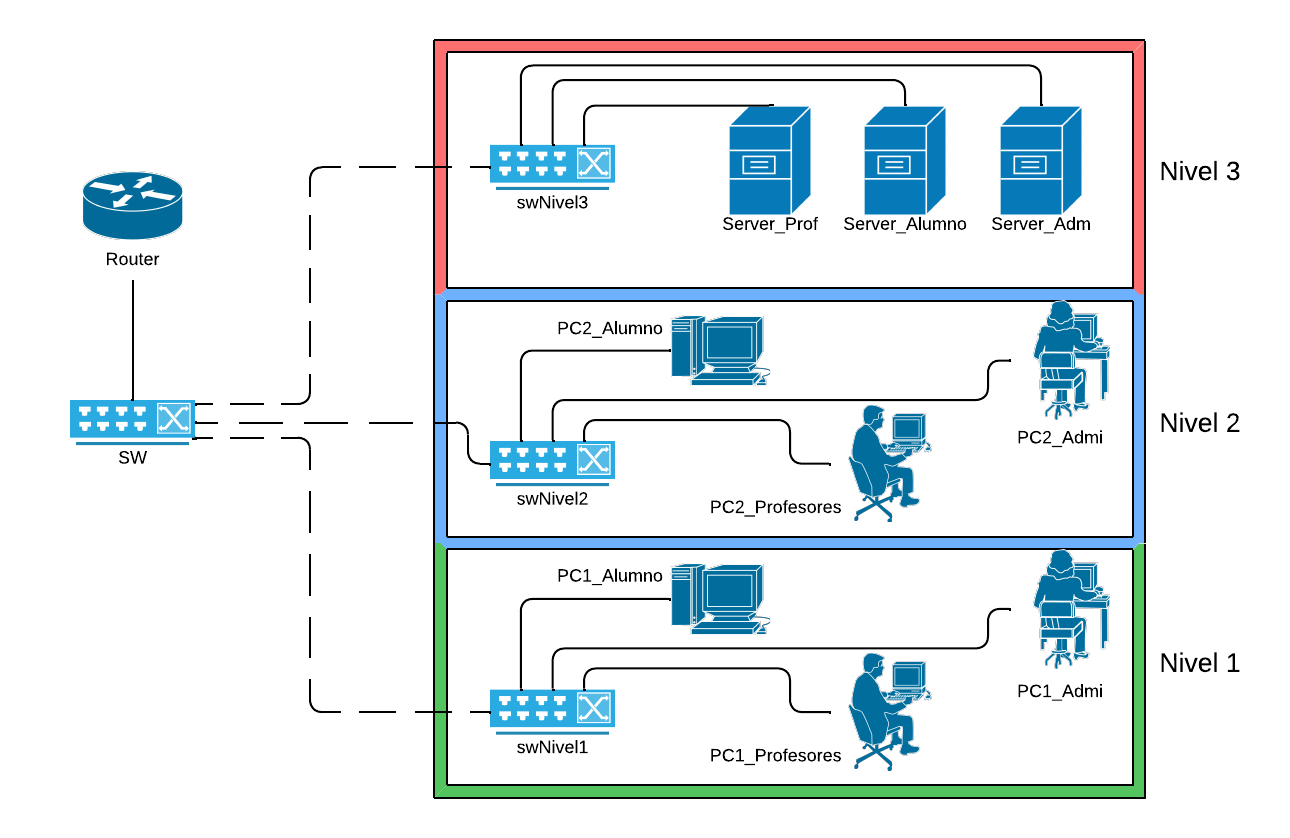
\includegraphics[width=0.6\textwidth]{img/topologia.png}
    \caption{Topología de la red}
    \label{fig:topologia}
\end{figure}

Los switches sugeridos por el consejo técnico del Instituto son cuatro serie 2960 de cisco modelo Ws-c2960 24lc-s y el router Serie 2900.

La asignación de puertos, de acuerdo con los requerimientos, es la siguiente:

\begin{enumerate}
    \item Puerto 1 a 7 para Profesores
    \item Puerto 8 a 15 para Alumnos
    \item Puerto 16 a 23 para Administrativos
\end{enumerate}

Además, durante el diseño se debe contemplar lo siguiente:

\begin{enumerate}
    \item [1] Proponga e implemente el diseño de la solución a este requerimiento en el simulador.
    \item [2] Realice la cotización del material y equipo a emplear. Recuerde que el Instituto ya cuenta con los equipos de cómputo.
    \item [3] Realice los planos de distribución (vista aérea y vista lateral).
\end{enumerate}

\section{Desarrollo del Trabajo}

    \subsection{Cálculo de Subredes}

    Para comenzar con el diseño de la red, se debe obtner las subredes necesarias para la red del instituto. Para ello, se debe calcular la cantidad de bits necesarios para la cantidad de dispositivos que se tienen en cada subred.

    \subsubsection*{Paso 1: Calcular la cantidad de subredes necesarias}

    \begin{equation}
        2^{n} \geq \text{Número de subredes} 
        \label{eq:subredes}
    \end{equation}

    \subsubsection*{Paso 2: Calcular el rango de direcciones IP}

    \subsubsection*{Paso 3: Obtener la IP de red y la IP de broadcast}

    \begin{table}[H]
        \begin{center}
            \begin{tabular}{ c | c | c | c | c }
                \textbf{Subred} & \textbf{VLAN} & \textbf{IP de Red} & \textbf{Broadcast} & \textbf{Puerto}\\ \hline
                1 & - & 192.168.10.0 & 192.168.10.63 & - \\
                2 & Profesores & 192.168.10.64 & 192.168.10.127 & 1 al 7\\
                3 & Alumnos & 192.168.10.128 & 192.168.10.191 & 8 al 15\\
                4 & Administrativos & 192.168.10.192 & 192.168.10.255 & 16 al 23\\
            \end{tabular}
            \caption{Subredes y VLANs}
            \label{tab:VLANs}
        \end{center}
    \end{table}

    \subsubsection*{Paso 4: Calcular la cantidad de hosts por subred}




\section{Conclusiones}
